\section{Aufbau und Durchführung}
\label{sec:Durchführung}

Der Versuchsaufbau ist in \autoref{fig:Abb_4} dargestellt.
\begin{figure}[H]
    \centering
    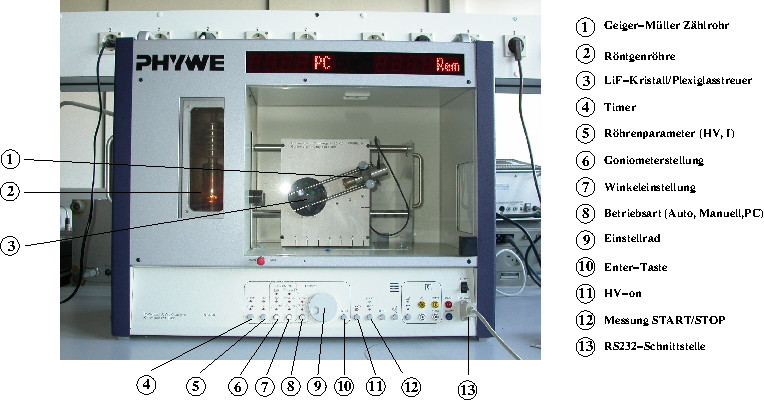
\includegraphics[width=\textwidth]{build/Abb_4.pdf}
    \caption{Versuchsaufbau und Benennung der Bestandteile.\cite{V602}}
    \label{fig:Abb_4}
\end{figure}

Die wesentlichen Bestandteile sind eine Kupfer-Röntgenröhre, ein LiF-Kristall und ein Geiger-Müller-Zählrohr.
Die Strahlung der Röntgenröhre ist auf den Kristall gerichtet, wobei dieser drehbar ist und somit die Intensität der 
Röntgenstrahlung durch das Geiger-Müller-Zählrohr für variierbare Glanzwinkel gemessen werden kann.
Mithilfe der Einstellelemente der Apparatur kann die Messung geregelt werden. Die Beschleunigungsspannung an der Röntgenröhre
wird für alle Messungen auf $U = \qty{35}{\kilo\volt}$ eingestellt und der Emissionsstrom am Geiger-Müller-Zählrohr auf $I = \qty{1}{\milli\ampere}$.
Mithilfe der Winkeleinstellung ($7$) kann ein fester Winkel für den LiF-Kristall eingestellt werden.
Die $\qty{1}{\milli\meter}$ Blende und der Kristall werden in die jeweiligen Halterungen gebracht.
Die Schlitzblende muss waagerecht auf dem Geiger-Müller-Zählrohr sitzen.
Die Messergebnisse werden über einen PC aufgenommen. 
Es kann die Messart, der Kristallwinkel, ein Drehmodus und die Integrationszeit für die Messungen ausgewählt bzw. eingestellt werden.
Als Messart wird "Spektren" verwendet.

\subsection{Überprüfung der Bragg-Bedingung} % (fold)
\label{sub:Bragg_durch}

Im ersten Versuchsteil wird die Bragg-Bedingung überprüft. Dazu wird ein fester Kristallwinkel von $\theta = \qty{14}{\degree}$ eingestellt.
Mit einem Winkelzuwachs von $\Delta\theta = \qty{0.1}{\degree}$ in einer Integrationszeit
von $\Delta t = \qty{5}{\second}$ wird die Intensität der Röntgenstrahlung am Geiger-Müller-Zählrohr in
einem Winkelbereich von $\theta_{GM} = \qty{26}{\degree}$ bis $\theta_{GM} = \qty{30}{\degree}$ gemessen.
Es wird eine 
% subsection Überprüfung der Bragg-Bedingung (end)

\subsection{Analyse des Emissionsspektrums einer Cu-Röntgenröhre} % (fold)
\label{sub:Emission_durch}

Um das Emissionsspektrum der Röntgenröhre aufzunehmen werden im Programm measure die Einstellungen verändert.
Die Messung erfolgt im 2:1 Koppelmodus. Das Röntgenspektrum wird im Winkelbereich von $\theta = \qty{26}{\degree}$ bis $\theta_{GM} = \qty{30}{\degree}$ gemessen. 


% subsection Das Emissionsspektrum einer Cu-Röntgenröhre (end)

\subsection{Analyse der Absorptionsspektren} % (fold)
\label{sub:Absorption_durch}

% subsection Das Absorptionsspektrum (end)